\pagebreak
\section{Vehicle's Inertia Test} \label{app:inertiaTest}
\textbf{Name: Group 510}\\
\textbf{Date: 02/11 - 2015}

\subsection{Purpose}
The purpose of the test is to measure the velocity system's time constant and find the inertia of the vehicle, \si{J_{tot}}, using this time constant.
\subsection{Theory}
%-- Not the right test anymore, but could still be useful in case we change our minds --%
% The \figref{inertiaTestPowerCutOrDisable} shows the vehicle's velocity variations throughout time, both when the motor is unplugged manually or when its power is cut via software :

% \begin{figure}[H]
%   \centering
%   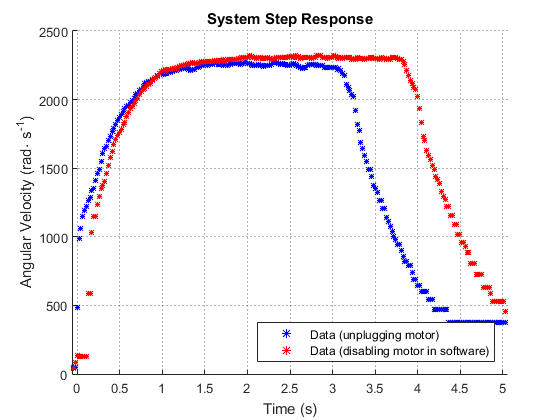
\includegraphics[scale=0.8]{figures/inertiaTestPowerCutOrDisable.png}
%   \caption{Plot of the systems step-response, which is angular velocity over time. The blue dots represents the measured data when the plus-pole of the motor is unplugged manually to stop the vehicle. The red dots represents the measured data when the software is used to stop the vehicle.}
%   \label{inertiaTestPowerCutOrDisable}
% \end{figure}

% By comparing both methods to cut off the motor's power, the back electromotive force generated by the motor when using the software method seems negligible since both curves have very similar decreasing shapes. Moreover, the manual unplugging of the powering wires brings some uncertainty due to a potential disturbance of the force applied to the vehicle.\\
% Therefore, the software method is used to extract the inertia.
%-- End of the first test version --%

\subsubsection{Using two steps}
In this test a two-step input is used to get the system's response. The reason for this is to avoid the stiction (also called Coulomb friction) when the vehicle starts. The second step input is not sent until the vehicle is in a steady and non-zero velocity. Without these two steps the first data points of the response are unusable, as seen in the results on \figref{fig:MomentOfInertiaTestPlot}.

\begin{figure}[H]
  \centering
  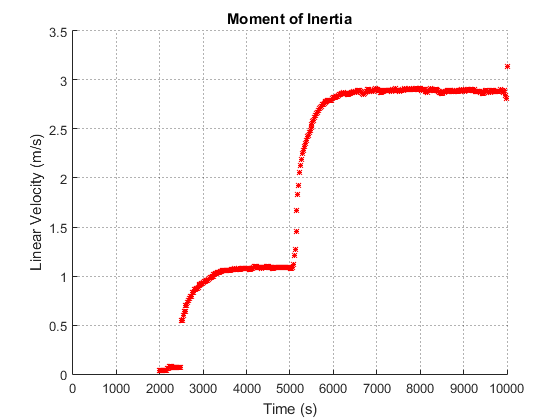
\includegraphics[scale=0.8]{figures/VehicleMomentOfInertiaTest.png}
  \caption{Vehicle's velocity response to a two-steps input}
  \label{fig:MomentOfInertiaTestPlot}
\end{figure}

%% Derivation of inertia formula %%
\subsubsection{Inertia formula}

From \figref{fig:BlockDiagramDrivetrainNotComplicated}, it is possible to neglect the motor's armature inductance, \si{L_a}, which is very small before the armature's resistance \si{R_a}, see \appref{app:motorTestArmatureResistance}. The derived simplified transfer function of the motorshaft's angular velocity, relative to the voltage input is then:
%-- Velocity model Tf with neglected La --%
\begin{flalign}
\eq{\frac{\omega(s)}{U_a(s)}}{\frac{\frac{K_t}{R_a} \cdot \frac{\frac{1}{B_{tot}}}{\frac{J_{tot}}{B_{tot}} \cdot s + 1}}{1 + \frac{K_t \cdot K_e}{R_a} \cdot \frac{\frac{1}{B_{tot}}}{\frac{J_{tot}}{B_{tot}} \cdot s + 1}}}&
\end{flalign}
\hspace{6mm} Where:\\
\begin{tabular}{p{1cm}lll}
& $J_{tot}$ & is the vehicle's total inertia                  &\unitWh{kg \cdot m^2}\\
& $B_{tot}$ & is the vehicle's total friction                 &\unitWh{N \cdot m \cdot s}\\
& $R_a$     & is the motor's armature resistance              &\unitWh{\Omega}\\
& $K_t$     & is the motor constant                           &\unitWh{Wb}\\
& $K_e$     & is the motor's generator constant               &\unitWh{Wb}\\
\end{tabular}
\todo{Do we use units in the Laplace domain ?}

This can be rewritten in the standard form as :
\begin{flalign}
\eq{\frac{\omega(s)}{U_a(s)}}{\frac{\frac{K_t}{B_{tot} \cdot R_a + K_t \cdot K_e}}{\frac{J_{tot} \cdot R_a}{B_{tot} \cdot R_a + K_t \cdot K_e} \cdot s + 1}}&
% \label{eq:velocityModelStandardNeglectedInductance}
\end{flalign}

That means that the time constant of the entire velocity model, \si{\tau}, can be expressed as:
\begin{flalign}
\eq{\tau}{\frac{J_{tot} \cdot R_a}{B_{tot} \cdot R_a + K_t \cdot K_e}} \unit{s}
\label{eq:velocityTimeConstant}
\end{flalign}

%-- Final inertia formula --%
Eventually, since the time constant is found by use of the system step response, it is possible to rearrange \eqref{eq:velocityTimeConstant} to obtain \si{J_{tot}}:
\begin{flalign}
\eq{J_{tot}}{\tau \cdot \left(B_{tot} + \frac{K_t \cdot K_e}{R_a}\right)} \unit{kg \cdot m^{2}}
\label{eq:inertiaFormula}
\end{flalign}

%% Test setup description %%
\subsection{Setup}
\begin{figure}[H]
	\centering
	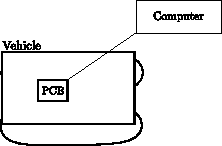
\includegraphics[scale=1.6]{figures/inertiaTestSetupDiagram2.pdf}
	\caption{Setup diagram}
	\label{inertiaTestSetupDiagram}
\end{figure}

\subsection{List of Equipment}

\begin{table}[H]
\begin{tabular}{|p{10cm}|p{4cm}|}
\hline%------------------------------------------------------------------------------------
  \textbf{Instrument}                     &  \textbf{Type}       \\
\hline%------------------------------------------------------------------------------------
  Computer                                &  Asus N73JN    \\
\hline %-----------------------------------------------------------------------------------
\end{tabular}
\end{table}

%% Procedure %%
\subsection{Procedure}

\begin{enumerate}
  \item Disconnect the battery.
  \item Connect the Arduino to the computer.
  \item Upload the test code to the Arduino board using the Arduino IDE  \cite{ArduinoIDE}.
  \item Open a serial terminal via PuTTY \cite{PuTTY}.
  \item Plug in the battery immediately after opening the terminal.
  \item Wait two seconds, then follow the vehicle with the connected computer.
  \item Wait until the vehicle stops before ending the measurements by unplugging the connected computer from the Arduino.
  \item Plot the speed of the vehicle using Matlab.
\end{enumerate}

%% Results %%
\subsection{Results} \label{inertiaTestResults}

\begin{figure}[H]
  \centering
  %Trim margins @:   left        bottom       right       top
  \adjustbox{ trim = {.15\width} {.30\height} {.15\width} {.30\height}, clip }
  {
    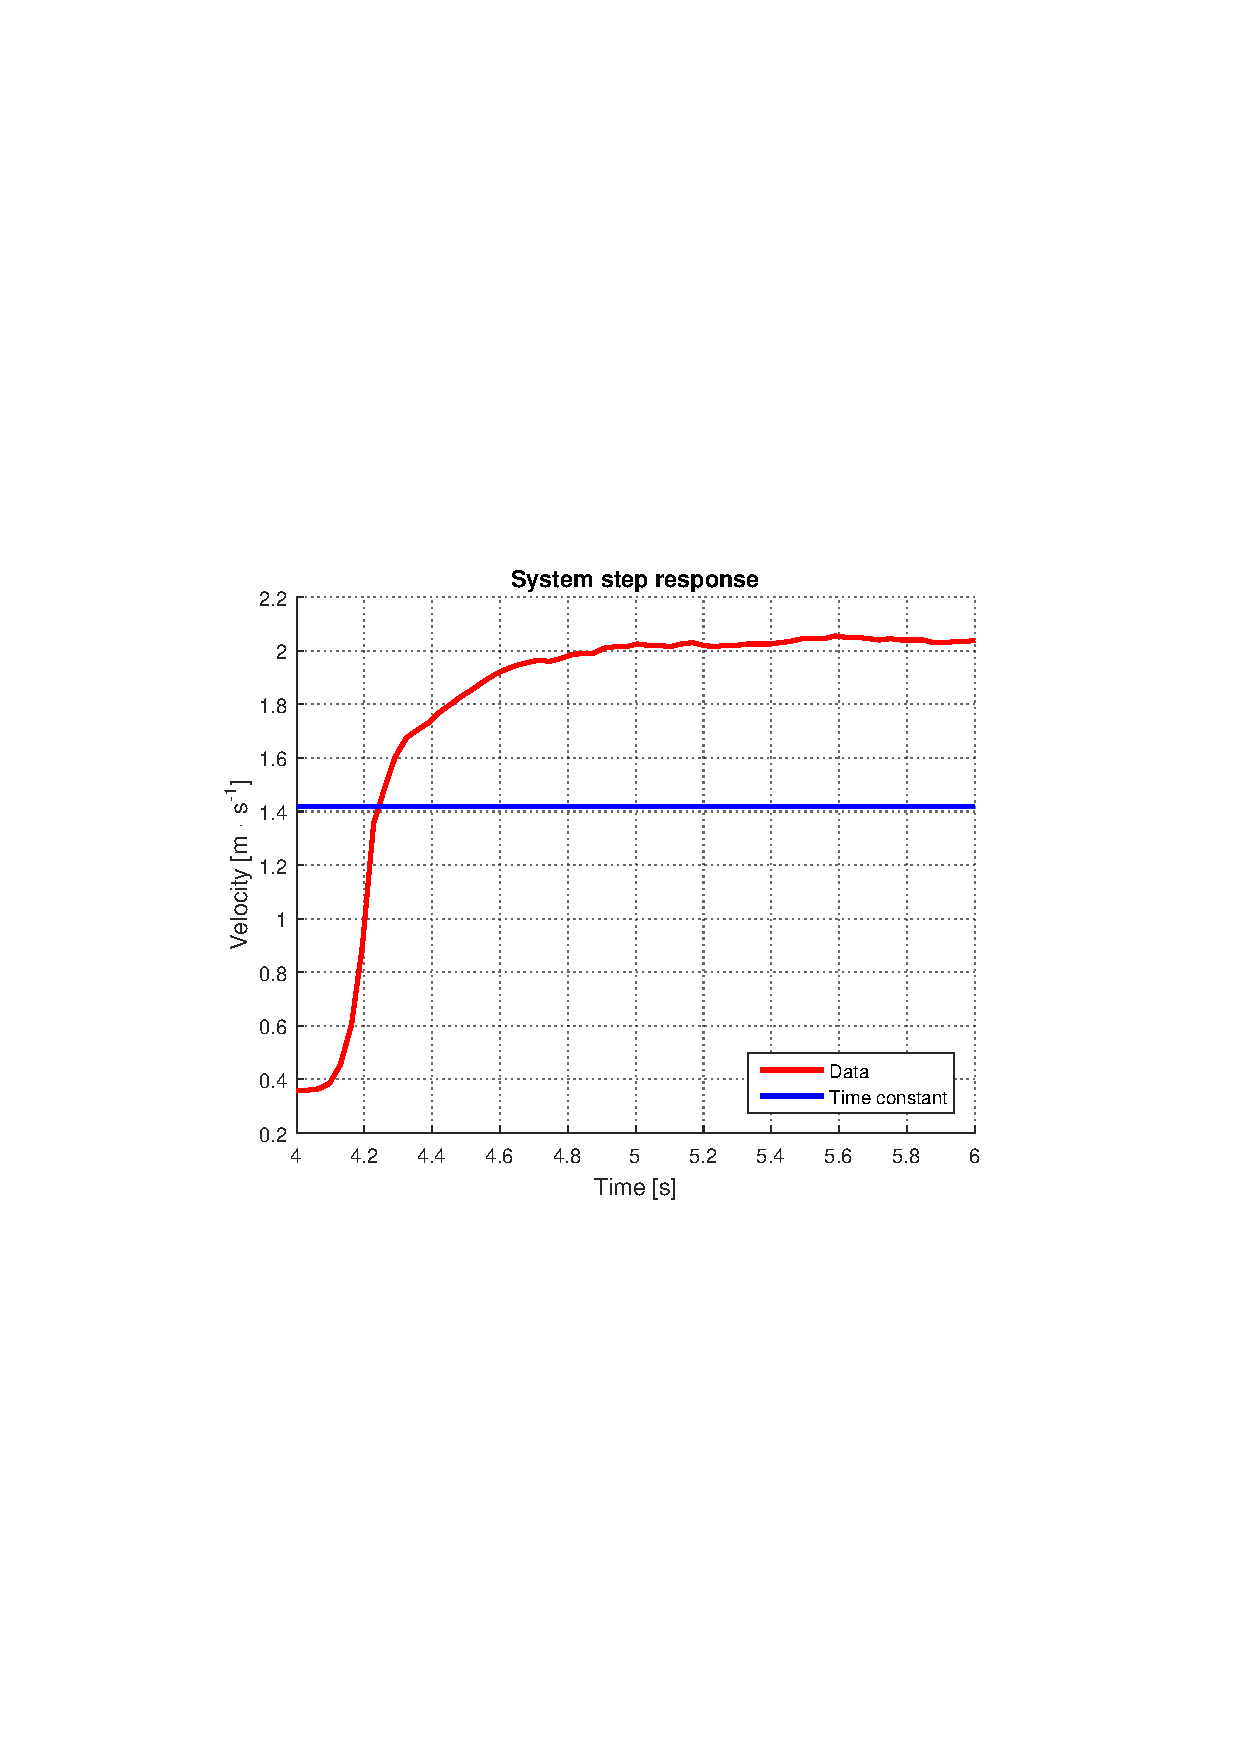
\includegraphics[width=1.0\textwidth]{figures/systemTimeConstant.pdf}
  }
  \caption{Time constant on a step-response}
  \label{fig:systemTimeConstant}
\end{figure}
%
In this test, a first voltage step is applied to the motor so that the vehicle runs at a minimal speed. A second bigger step is then applied. The analyzed data is the one retrieved between these two steps and it can be seen on \figref{fig:systemTimeConstant}. A blue line is drawn at \si{\num{63,2} \%} of the final velocity.

%- Time constant -% 
\subsubsection{Velocity System's Time Constant}
Only, the second step is used. By knowing the maximum velocity of the vehicle at the end of the test and the velocity when it is in a first steady state, just before the second step, it is possible to deduce the time at which the velocity reaches \si{\num{63,2} \%} of its final value. The obtained time is the step response time constant of the system \si{\tau}.

Since the velocity is taken at \si{\num{63,2} \%} between the first steady state and the final value, it is needed to shift it up with the starting value \si{V_{ss1}} :
\begin{flalign}
\eq{V(\tau + t_0)}{(V_{max} - V_{ss1}) \cdot 0,632 + V_{ss1}} \unit{m \cdot s^{-1}}
\end{flalign}
\hspace{6mm} Where:\\
\begin{tabular}{p{1cm}lll}
& $V(\tau + t_0)$ & is the velocity at \si{\num{63,2} \%} of the final velocity       &\unitWh{m \cdot s^{-1}}\\
& $t_0$           & is the time at which the second step starts                       &\unitWh{s}\\
& $V_{max}$       & is the maximum velocity                                           &\unitWh{m \cdot s^{-1}}\\
& $V_{ss1}$       & is the velocity in steady state corresponding to the first step   &\unitWh{m \cdot s^{-1}}\\
\end{tabular}

%to find tau:
%read average speed before and after the step
%after:  2.04m/s
%before: 0.36m/s
%delta = 2.04-0.36 = 1.68
%tau is at 63.2% of the delta + the start speed: 1.68*0.632 + 0.36 =
%1.06m/s + 0.36m/s = 1.42m/s
%reading the time we crosss 1.42m/s: 4.243 seconds
%step starts at 4.032 seconds
%tau is therefore 4.243-4.032 = 0.211 seconds


According to the data, the velocity of the vehicle at that point is :
\begin{flalign}
  \eq{V(\tau + t_0)}{\left(2,04 - 0,36\right) \cdot 0,632 + 0,36}&\nonumber
  \eq{V(\tau + t_0)}{1,42} \si{\ m \cdot s^{-1}}&\nonumber
\end{flalign}
%
The corresponding time stamp to that velocity \si{t_1} is:
\begin{flalign}
  \eq{t_1}{4,243} \si{\ s}&\nonumber
\end{flalign}
%
However, it is also needed to shift down the time scale so that the time \si{t_0} at which the second step begins is the time origin :
%
\begin{flalign}
\eq{\tau}{t_1 - t_0} \unit{s}
\end{flalign}
% \hspace{6mm} Where:\\
% \begin{tabular}{p{1cm}lll}
% & $t_1$   & is the time at which \si{\num{63,2} \%} of the final value have been reached  &\unitWh{s}\\
% \end{tabular}


Therefore, the time constant is: 
\begin{flalign}
\eq{\tau}{4,243 - 4,032}&\nonumber\\
  % &\Updownarrow&\nonumber\\
\eq{\tau}{0,211} \si{\ s}&\nonumber
\end{flalign}

%- Inertia calculation -%
\subsubsection{Total Inertia Calculation}
%
Eventually, the \eqref{eq:inertiaFormula} is used to calculate \si{J_{tot}}. Using values found in previous tests leads to \si{J_{tot}} being :
\begin{flalign}
\eq{J_{tot}}{4,5782 \cdot 10^{-6}} \si{\ kg \cdot m^2}&\nonumber
\end{flalign}